\documentclass[crop, tikz]{standalone}


\usepackage{tikz}
\usepackage{tikz-dimline}
\usetikzlibrary{shapes,arrows,shadows}
\usepackage{amsmath,bm,times}
\begin{document}
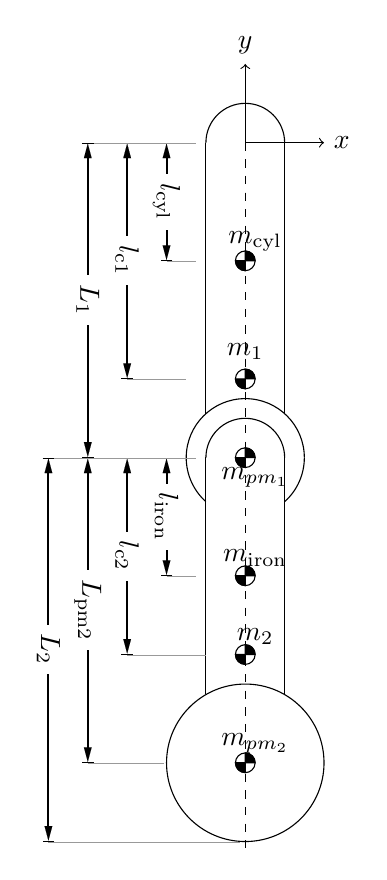
\begin{tikzpicture}[scale=0.5]




\begin{scope}
\clip [rotate=0] (-2,0) rectangle (2,2);
\draw (0,0) circle [radius=1cm];
\end{scope}

\coordinate (O) at (0,0) ;
% Second cirle middle point
\coordinate (A) at (3.5,-6.06217); 
\coordinate (B) at (3.5+6.06217,-6.06217-3.5);
\coordinate (L1) at (0,-6);
\coordinate (L2) at (0,-14);
\coordinate (x) at (0,-2);
\coordinate (AA) at ([xshift=-1cm]x);
\coordinate (BB) at ([xshift=1cm]x);
\coordinate (CC) at ([xshift=1cm,yshift=-1.5cm]x);
\coordinate (DD) at ([xshift=-1cm,yshift=-1.5cm]x);

	% Lenght of pendulums are 7cm

	% Axis for underactuated Pendulum
	\draw[->] (0,0) -- (2,0) node[anchor=west] {$x$};
	\draw[->] (0,0) -- (0,2) node[anchor=south] {$y$};
	\draw[dashed] (0,0) -- (0,-2);
	
	%%%%%%%%%%%%%%%%%%%%%%%%%%%%%%%%%%%%%%%%%%%%%%%%%%%%%%%%%%%%%%%%%%%%%%%%%%%%%%

	%%%%%%%%%%%%%%%%%%%%%%%%%%%%%%%%%%%%%%%%%%%%%%%%%%%%%%%%%%%%%%%%%%%%%%%%%%%%%%
	
	%%%%%%%%%%%%%%%%%%%%%%%%%%%%%%%%%%%%%%%%%%%%%%%%%%%%%%%%%%%%%%%%%%%%%%%%%%%%%%
				%% Middle line for underactuated pendulum %%
	\draw[dashed] (O) -- ([yshift=-4cm]L2);
	%%%%%%%%%%%%%%%%%%%%%%%%%%%%%%%%%%%%%%%%%%%%%%%%%%%%%%%%%%%%%%%%%%%%%%%%%%%%%%
	
		
	%%%%%%%%%%%%%%%%%%%%%%%%%%%%%%%%%%%%%%%%%%%%%%%%%%%%%%%%%%%%%%%%%%%%%%%%%%%%%%
					%% Dimensions of underactuated Pendulum %%
	\dimline[line style = {line width=0.7},extension start length=-0.25, extension end length=-0.25]{(-2,0)}{(-2,-3)}{$l_{\text{cyl}}$}
	
	\dimline[line style = {line width=0.7},extension start length=-0.25, extension end length=-0.25]{(-3,0)}{(-3,-6)}{$l_{\text{c1}}$}
	
	\dimline[line style = {line width=0.7},extension start length=-0.25, extension end length=-0.25]{(-4,0)}{(-4,-8)}{$L_{1}$}
	
	%%%%%%%%%%%%%%%%%%%%%%%%%%%%%%%%%%%%%%%%%%%%%%%%%%%%%%%%%%%%%%%%%%%%%%%%%%%%%%

	%Long lines for underactuated pendulum
	\draw[] (-1,0) -- ([xshift=-1cm,yshift=-0.9cm]L1);
	\draw[] (1,0) -- 	([xshift=1cm,yshift=-0.9cm]L1);	
	
	
	
	%%%%%%%%%%%%%%%%%%%%%%%%%%%%%%%%%%%%%%%%%%%%%%%%%%%%%%%%%%%%%%%%%%%%%%%%%%%%%%
					%% smaller Middle circle for both pendulums %
	\begin{scope}
	\clip ([xshift=-1.2cm,yshift=-2cm]L1) rectangle ([xshift=1.2cm,yshift=2cm]L1);
	\draw ([yshift=-2cm]L1) circle [radius=1cm];
	\end{scope}
	
	
	% Bigger Middler Circle for both pendulums
	%\draw ([yshift=-2cm]L1) circle [radius=1.5cm];
	\draw[] ([xshift=1.5cm,yshift=-2cm]L1)
	arc[start angle = 0, end angle = 228, radius = 1.5cm];
	
	\draw[] ([xshift=1.5cm,yshift=-2cm]L1)
	arc[start angle = 0, end angle =-48 , radius = 1.5cm];

	%\draw [rotate=00] (0.866+3.5,0.5-6.06217+2) rectangle (-0.866+3.5-2,-0.5-6.06217);
	
	%%%%%%%%%%%%%%%%%%%%%%%%%%%%%%%%%%%%%%%%%%%%%%%%%%%%%%%%%%%%%%%%%%%%%%%%%%%%%%

	\begin{scope}
	\clip ([xshift=-1.5cm,yshift=-2cm]L1) rectangle ([xshift=1.5cm,]L2);
	\draw[] ([xshift=-1cm,yshift=-1.5cm]L1) --([xshift=-1cm]L2);
	\draw[]([xshift=1cm,yshift=-1.5cm]L1) --([xshift=1cm,]L2);
	\end{scope}
	
	
	%%%%%%%%%%%%%%%%%%%%%%%%%%%%%%%%%%%%%%%%%%%%%%%%%%%%%%%%%%%%%%%%%%%%%%%%%%%%
	
	%%%%%%%%%%%%%%%%%%%%%%%%%%%%%%%%%%%%%%%%%%%%%%%%%%%%%%%%%%%%%%%%%%%%%%%%%%%%%%
	
	%%%%%%%%%%%%%%%%%%%%%%%%%%%%%%%%%%%%%%%%%%%%%%%%%%%%%%%%%%%%%%%%%%%%%%%%%%%%%%
						%% Dimensions of actuated Pendulum %%
	\dimline[line style = {line width=0.7},extension start length=-0.25, extension end length=-0.25]{(-2,-8)}{(-2,-11)}{$l_{\text{iron}}$}
	
	\dimline[line style = {line width=0.7},extension start length=-0.25, extension end length=-0.4]{(-3,-8)}{(-3,-13)}{$l_{\text{c2}}$}
	
	\dimline[line style = {line width=0.7},extension start length=-0.25, extension end length=-0.25]{(-4,-8)}{(-4,-15.75)}{$L_{\text{pm2}}$}
	
	
	\dimline[line style = {line width=0.7},extension start length=-0.25, extension end length=-0.5]{(-5,-8)}{(-5,-17.75)}{$L_{2}$}
	%%%%%%%%%%%%%%%%%%%%%%%%%%%%%%%%%%%%%%%%%%%%%%%%%%%%%%%%%%%%%%%%%%%%%%%%%%%%%%

	
	%%%%%%%%%%%%%%%%%%%%%%%%%%%%%%%%%%%%%%%%%%%%%%%%%%%%%%%%%%%%%%%%%%%%%%%%%%%%%%
							%% Circle at the bottom %%
	\draw ([yshift=-1.75cm]L2) circle [radius=2cm];
	%%%%%%%%%%%%%%%%%%%%%%%%%%%%%%%%%%%%%%%%%%%%%%%%%%%%%%%%%%%%%%%%%%%%%%%%%%%%%%

	
	%%%%%%%%%%%%%%%%%%%%%%%%%%%%%%%%%%%%%%%%%%%%%%%%%%%%%%%%%%%%%%%%%%%%%%%%%%%%%%


	%%%%%%%%%%%%%%%%%%%%%%%%%%%%%%%%%%%%%%%%%%%%%%%%%%%%%%%%%%%%%%%%%%%%%%%%%%%%%%
				%% Centroid symbol for underactuade pendulum %%
	\draw (0,-6) circle [radius=0.25cm];
	\draw (0,-6-0.25) -- (0,-6+0.25)  node[above]{$m_{1}$};`
	\draw (0,-6+0.25) -- (0,-6-0.25);
	\filldraw[fill=black,draw=black] (0,-6) -- (0.25,-6)
		arc[start angle = 0, end angle = 90, radius = 0.25] -- cycle;
		
	\filldraw[fill=black,draw=black] (0,-6) -- (-0.25,-6)
	arc[start angle = 180, end angle = 270, radius = 0.25] -- cycle ;
	%%%%%%%%%%%%%%%%%%%%%%%%%%%%%%%%%%%%%%%%%%%%%%%%%%%%%%%%%%%%%%%%%%%%%%%%%%%%%%
	
	%%%%%%%%%%%%%%%%%%%%%%%%%%%%%%%%%%%%%%%%%%%%%%%%%%%%%%%%%%%%%%%%%%%%%%%%%%%%%%
				%% Centroid symbol for actuaded pendulum %%
	\draw (0,-13) circle [radius=0.25cm];
	\draw (-0.25,-13) -- (0.25,-13)  node[above]{$m_{2}$};
	\draw (0,-13+0.25) -- (0,-13-0.25);
	\filldraw[fill=black,draw=black] (0,-13) -- (0.25,-13)
	arc[start angle = 0, end angle = 90, radius = 0.25] -- cycle;
	
	\filldraw[fill=black,draw=black] (0,-13) -- (-0.25,-13)
	arc[start angle = 180, end angle = 270, radius = 0.25] -- cycle ;
	%%%%%%%%%%%%%%%%%%%%%%%%%%%%%%%%%%%%%%%%%%%%%%%%%%%%%%%%%%%%%%%%%%%%%%%%%%%%%%
				%% Centroid symbol for pointmass 2 %%
\draw (0,-15.75) circle [radius=0.25cm];
\draw (-0.25,-15.75) -- (0.25,-15.75)  node[above]{$m_{\text{$pm_2$}}$};
\draw (0,-15.75+0.25) -- (0,-15.75-0.25);
\filldraw[fill=black,draw=black] (0,-15.75) -- (0.25,-15.75)
arc[start angle = 0, end angle = 90, radius = 0.25] -- cycle;

\filldraw[fill=black,draw=black] (0,-15.75) -- (-0.25,-15.75)
arc[start angle = 180, end angle = 270, radius = 0.25] -- cycle ;
	%%%%%%%%%%%%%%%%%%%%%%%%%%%%%%%%%%%%%%%%%%%%%%%%%%%%%%%%%%%%%%%%%%%%%%%%%%%%%%
				%% Centroid symbol for pointmass 1 %%
\draw (0,-8) circle [radius=0.25cm];
\draw (-0.25,-8) -- (0.25,-8)  node[below]{$m_{\text{$pm_{1}$}}$};
\draw (0,-8+0.25) -- (0,-8-0.25);
\filldraw[fill=black,draw=black] (0,-8) -- (0.25,-8)
arc[start angle = 0, end angle = 90, radius = 0.25] -- cycle;

\filldraw[fill=black,draw=black] (0,-8) -- (-0.25,-8)
arc[start angle = 180, end angle = 270, radius = 0.25] -- cycle ;
	%%%%%%%%%%%%%%%%%%%%%%%%%%%%%%%%%%%%%%%%%%%%%%%%%%%%%%%%%%%%%%%%%%%%%%%%%%%%%%
				%% Centroid symbol for cylinder %%
\draw (0,-3) circle [radius=0.25cm];
\draw (-0.25,-3) -- (0.25,-3)  node[above]{$m_{\text{cyl}}$};
\draw (0,-3+0.25) -- (0,-3-0.25);
\filldraw[fill=black,draw=black] (0,-3) -- (0.25,-3)
arc[start angle = 0, end angle = 90, radius = 0.25] -- cycle;

\filldraw[fill=black,draw=black] (0,-3) -- (-0.25,-3)
arc[start angle = 180, end angle = 270, radius = 0.25] -- cycle ;
%%%%%%%%%%%%%%%%%%%%%%%%%%%%%%%%%%%%%%%%%%%%%%%%%%%%%%%%%%%%%%%%%%%%%%%%%%%%%%
				%% Centroid symbol for iron ron %%
\draw (0,-11) circle [radius=0.25cm];
\draw (-0.25,-11) -- (0.25,-11)  node[above]{$m_{\text{iron}}$};
\draw (0,-11+0.25) -- (0,-11-0.25);
\filldraw[fill=black,draw=black] (0,-11) -- (0.25,-11)
arc[start angle = 0, end angle = 90, radius = 0.25] -- cycle;

\filldraw[fill=black,draw=black] (0,-11) -- (-0.25,-11)
arc[start angle = 180, end angle = 270, radius = 0.25] -- cycle ;


	
\end{tikzpicture}
\end{document}